\section{The {\famsec} Framework}
    \begin{figure}[tbp]
        \centering
        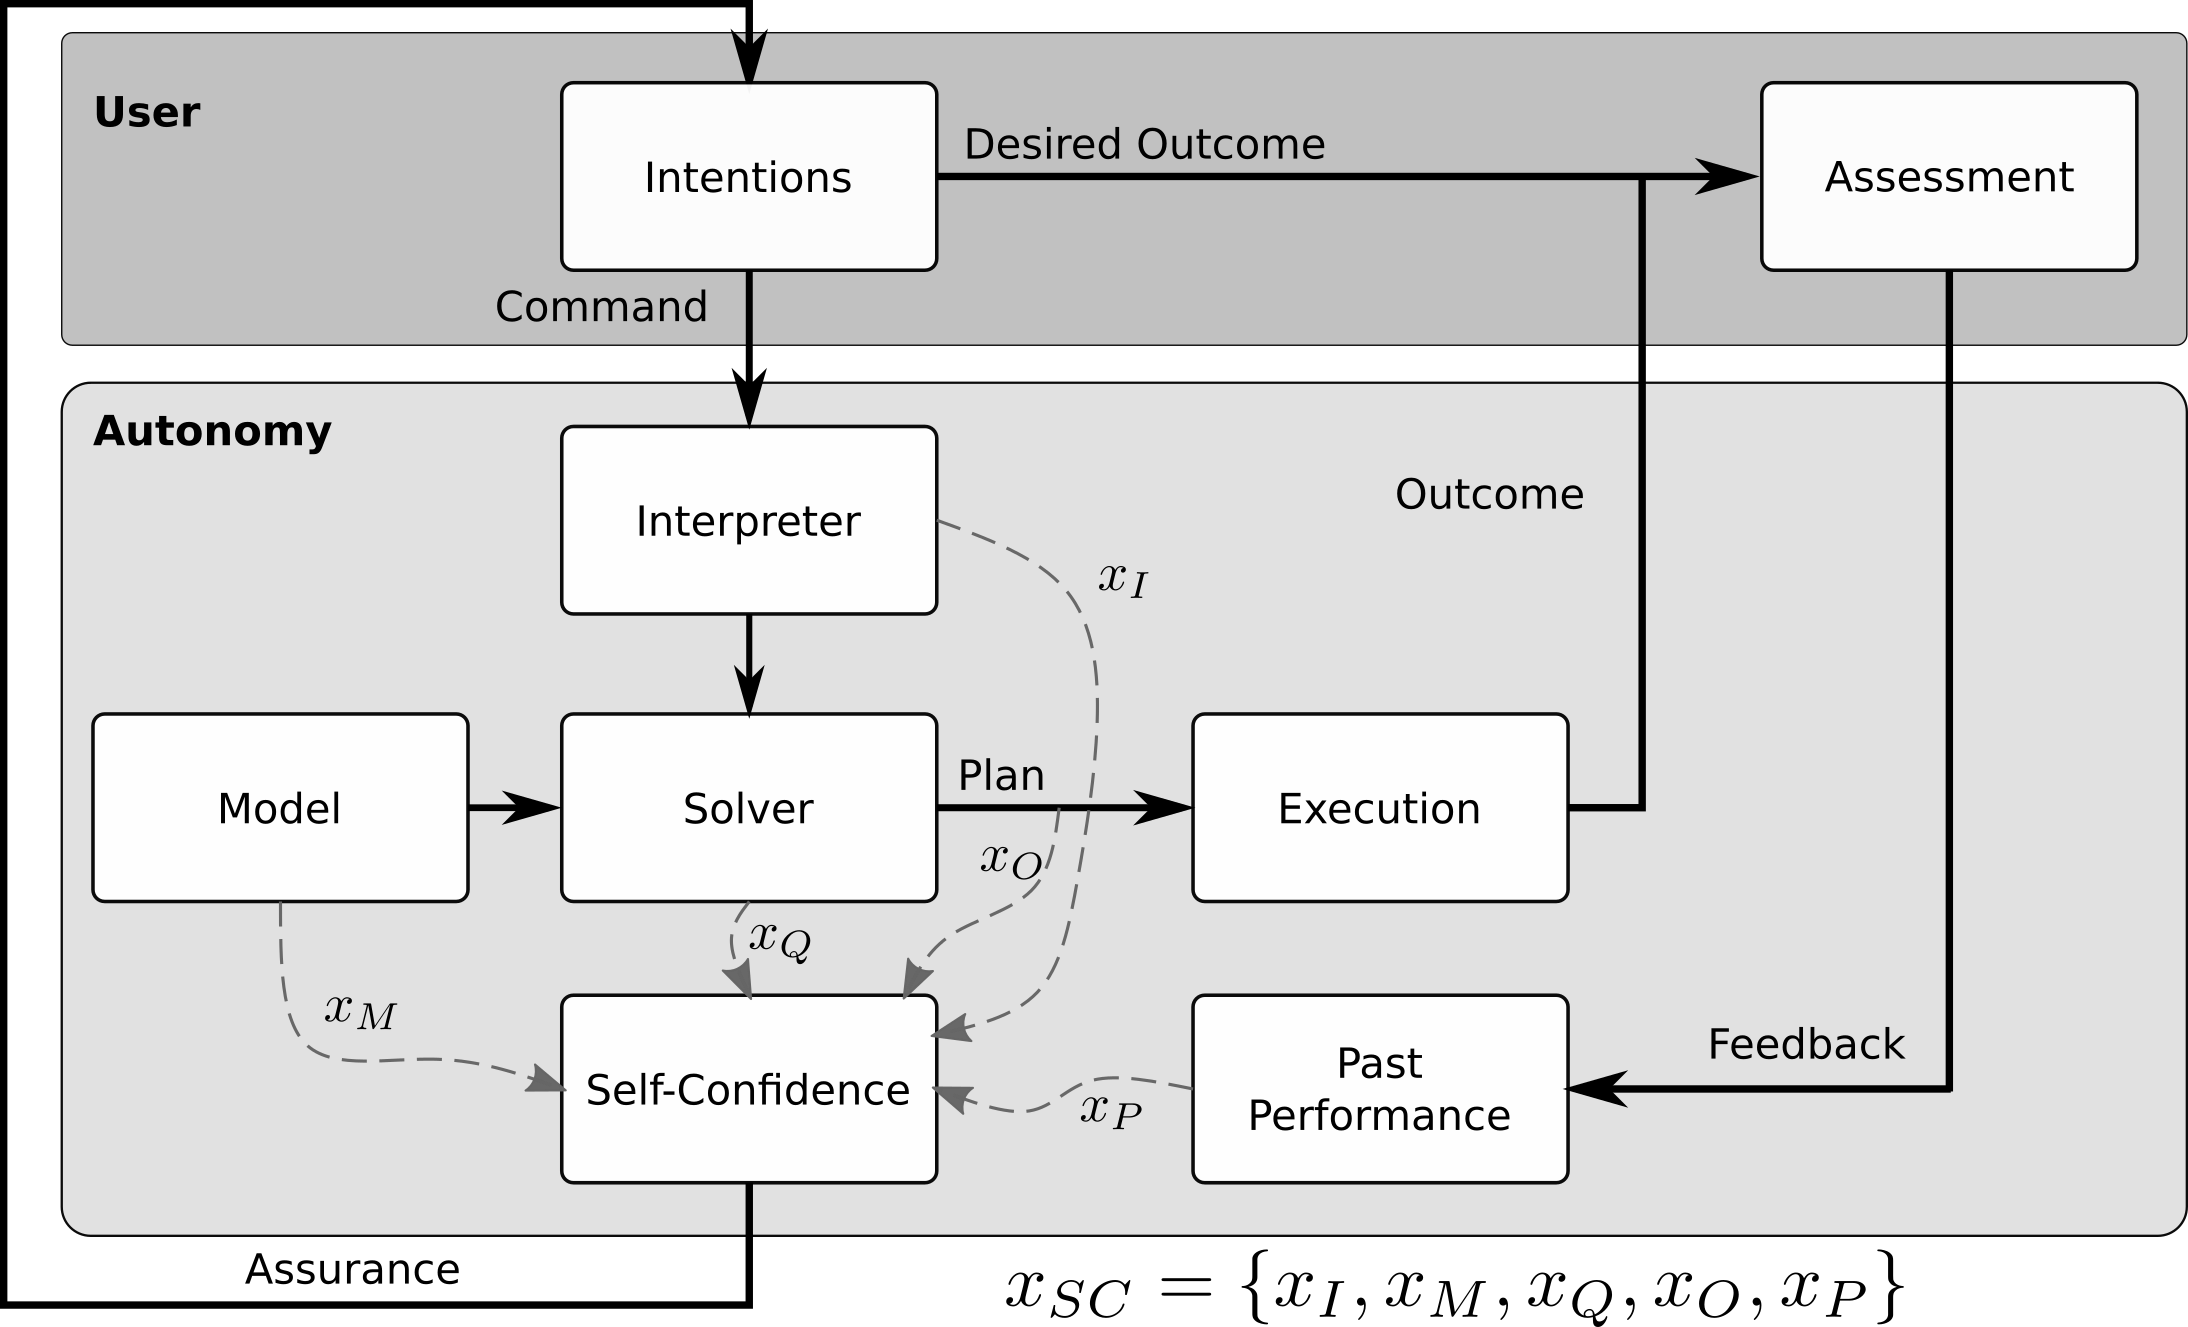
\includegraphics[width=0.95\linewidth]{Figures/FaMSeC.png}
        \caption{Factorized Machine Self-Confidence (FaMSeC)}
        \label{fig:famsec}
    \end{figure}
    
    This work seeks to develop an algorithmic framework for assessing and communicating machine self-confidence that endows an APS with a model-based process-driven understanding of how it arrives at decisions, and what factors influence the quality of its reasoning, in order to quantitatively assess its own competency boundaries. The approach taken here is motivated by the need to establish both: (i) a formal set of principles, definitions, and relations that govern the `arithmetic of machine self-confidence' as a function of task, environment, system realization, and context, and (ii) variables, representations and operations for producing meaningful self-confidence assessments. As such, this work initially addresses these issues for APS that are primarily defined by capabilities for dynamic decision-making and planning under uncertainty. This focused approach provides a pathway to developing firm initial mathematical and computational bases for addressing (i) and (ii) via the rich set of analytical and computational features inherent to the MDP model family. Insights developed along these lines will be extended in future work to other important APS capabilities that are formally related to decision making under uncertainty, such as dynamic learning and partially observable planning with sensing and perception. 
    
    ...\nisar{edit:} The approach adopted here builds on the \emph{Factorized Machine Self-Confidence (\famsec)} framework developed in ref. \cite{Aitken2016-cv, Aitken2016-fb}. The key idea behind \famsec is to represent and compute self-confidence as a traceable multi-factor function, which combines shorthand assessments of where and when operations and approximations inherent to model-based autonomous decision-making are expected to break down. As with the self-confidence reporting strategy developed by Hutchins, et al. in \cite{Hutchins2015-if}, this captures metrics than an expert designer would use to assess the correctness and quality of an autonomous decision-making system, accounting for variations in task, environment, system implementation, and context. However, unlike \cite{Hutchins2015-if}, \famsec allows an APS to automatically generate its own holistic assessments of self-confidence, i.e. without the need for a human designer/expert to specify a priori how self-confident a system ought to be in light of these same variations (which can be cumbersome, if not impossible, to fully account for in practical applications). 
    
    The block diagram in Figure \ref{fig:famsec} illustrates \famsec's notional overall self-confidence scoring mechanism. This uses a distinct set of \emph{self-confidence factors} (dashed lines) that are derived from core algorithmic decision-making components (white boxes in the `Autonomy' block). For concreteness and illustration purposes, the total self-confidence score can be mapped onto an arbitrary scale, e.g. -1 to +1, where -1 gives a shorthand indication of `complete lack of confidence' (i.e. some aspect of task, environment, or context falls completely outside the system's competency boundaries), and +1 indicates `complete confidence' (i.e. all aspects of task, environment, and mission context are well within system's competency boundaries). As will be shown later, the scales for each factor need not all be the same and can carry slightly different qualitative interpretations, as long as a clear sense of `confidence direction' (i.e. degree of self-trust) can be established for each. Ref. \cite{Aitken2016-cv} considers five general (though not necessarily exhaustive or exclusive) factors that contribute to a `total self-confidence score', which notionally maps the multivariate the combined set of individual factors into an overall confidence report:
    
    
\begin{enumerate}
\item \xI -- \textit{\textbf{interpretation of user intent and task}}: To what extent were the user's intentions properly understood and translated by the autonomous system into context-appropriate mission specifications and tasks? 
%This factor derives from features and parameters of the `Interpreter' block. 
For instance, if a natural language interface is used for mission planning, this factor could assess how well user inputs are mapped to reward functions using fixed vocabularies for different mission profiles. 
%This factor can, for instance, capture uncertainty in task objectives or reward functions \cite{abbeel2004apprenticeship, hadfield2016cooperative}. 
%
\item \xM -- \textit{\textbf{model and data validity}}: Are the agent's learned/assumed models and associated training data used for decision-making good enough proxies for the real world? This factor assesses how well the set of measurements and events predicted by the autonomous system line up with what it actually should observe in reality. 

%Specifically, this factor uses features and parameters of the `Model' block to assess how well the set of measurements and events predicted by the autonomous system line up with what it actually should observe in reality. 
%For the U2R2 problem, model validity is related to the size of the state space of the model and the level of discretization used in the environment and action set.
%
\item \xQ -- \textit{\textbf{solver quality}}: Are the approximations and learning-based adaptations used by the system for solving decision-making problems appropriate for the given mission and model? 
%%This factor uses features and parameters of the `Solver' block to assess the ability of the system to make appropriate decisions based on the information it is given. This factor directly assesses a key aspect of the inherent fitness of the reasoning process: s
Since approximations are almost always needed to solve otherwise intractable decision making problems,  this factor examines the appropriateness and reliability of those approximations. 
%For instance, if it is too costly to implement optimal planning, certain problem constraints can often be relaxed to arrive at nearly optimal decisions more cheaply; if such approximations are invalid in critical portions of the problem space, then these can result in poor decisions and hence low confidence in the solution quality. 
This factor also accounts for the impact of learning mechanisms required to make complex decisions under uncertainty, e.g. based on suitability of training data or the learning process to solving the problem at hand. 
%%\nraComm{Ufuk: here is the hook to talk about assessment of learning in MDP families...}
%For the U2R2 problem we will use a priori bounds on the optimality of the resulting policy given known properties of the model and data.
%
\item \xO-- \textit{\textbf{expected outcome assessment}}: Do the sets of possible events, rewards, costs, utilities, etc. for a particular decision lead to desirable outcomes? 
Even if the autonomous system perfectly understands and analyzes a mission, and can arrive at globally optimal solutions, it may still not be able to always avoid running into undesirable states along the way. % (e.g. due to the existence of catastrophic events with small but non-zero probabilities). 
This factor evaluates the particular decision making strategy implemented by the system to assess the inherent favorability of the full landscape of possible task outcomes.  
%For stochastic policies we use a variation of the upside potential ratio to assess the expected outcome. This measure is further weighted to account for known human biases at extreme outcome probabilities [XYZ]. 
%
\item \xP-- \textit{\textbf{past history and experiences}}: What can be gleaned from the system's own experience and other available historical information for past problem instances?  
This factor notionally allows the autonomous system to predict, transfer, and update assessments of self-confidence based on prior experiences, and thus embodies meta-memory and meta-learning for enabling and improving self-proficiency assessments. 
%For the U2R2 problem we use a combination of the current learned policy and the rate of change of the policy around the current state to determine how past performance should correlate with current behavior. 
\end{enumerate}
    
    
    Since the overall self-confidence mapping is heavily dependent on application, context, and desired levels/types of user-autonomy interaction, it is assumed for simplicity in this work that the overall mapping consists of a direct report of some fixed subset of the component factors, i.e. \xSC. 
    %%Incidentally, these characteristics of self-confidence (i.e. self-trust) component factors are not dissimilar from the multidimensional and contextual nature of the component factors that comprise human trust. 

        

    \nisar{edit...} Self-confidence \xSC{} is a composite assurance \nisar{do we need more jargon?} that stems from some combination of these five factors. \xP{} has been previously defined in \cite{Aitken2016-cv}, but has not yet been evaluated as an effective assurance as per the guidelines laid out in the work on assurances. Herein \xQ{} is investigated. \nisar{edit...note that we are notionally using -1 to 1 range as a notional example here...do we later shift this range to 0 to 2 for \xQ?? (maybe note this here...or just change in table example below -- and/or maybe use this to underscore fact that ranges can be set arbitrarily and depending on context, e.g. see Hutchins paper...don't want to get too hung up on this...) }

\subsection{VIP Escort Example Revisited}
\nisar{TODO: talk about possible stochastic motion planning solvers (could be MDP family or others...) and discuss/move in table with example boundary conditions -- BE MINDFUL OF RANGE VALUES AS PER NOTE ABOVE...transition to talking about computation: start with pointing to Matt's thesis work for outcome assessment with brief mention of UPM/LPM...then transition to next section on how to compute solver quality}

\begin{figure}[tbp]
    \centering
    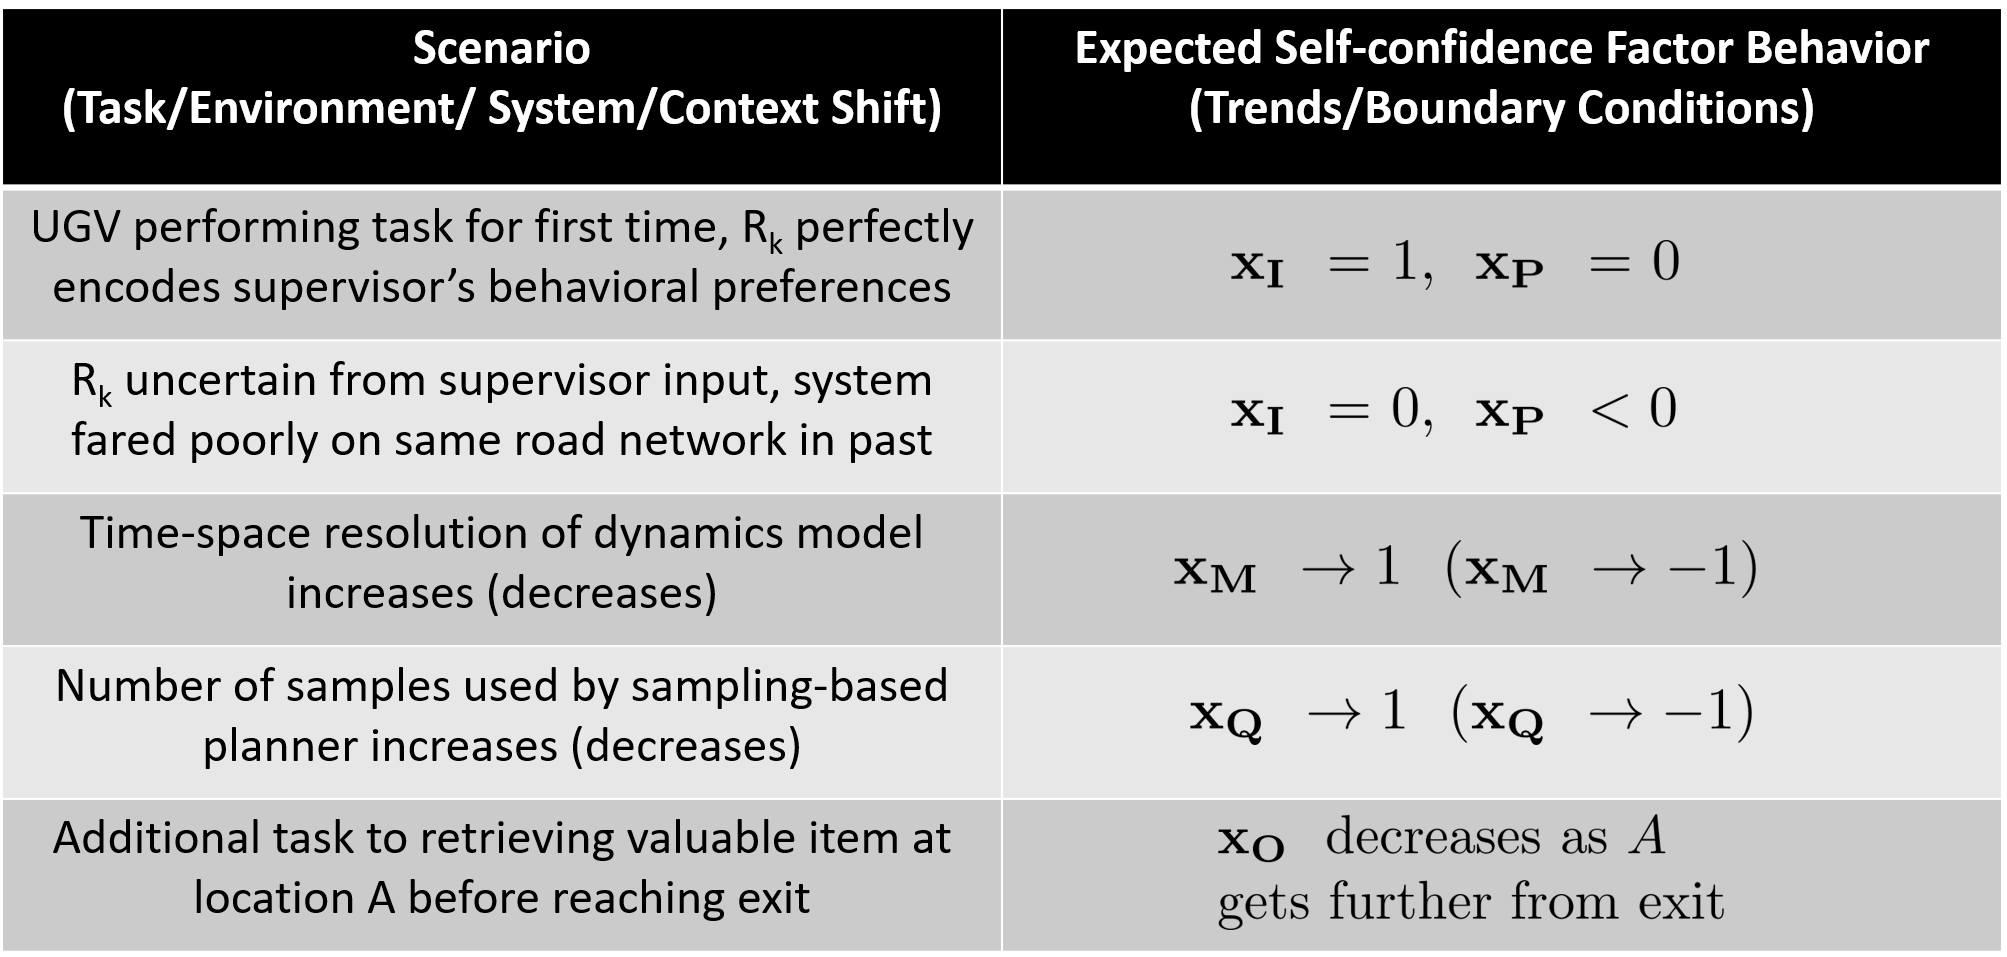
\includegraphics[width=0.99\linewidth]{Figures/scTrendsBoundaryExample.png}
    \caption{Notional \famsec behaviors for VIP Escort problem with a hypothetical stochastic planner.}
    \label{fig:roadnet}
    \vspace{-0.3 in}
\end{figure}

\subsection{Solver Quality (\xQ)} \label{sec:SQ}
    The main aim of \xQ{} is to indicate how a solver \solve{} will perform on a given (possibly un-encountered) task \task{}. Formally, the desiderata are:

    \begin{enumerate}[label=\textbf{D\arabic*}]
        \item reflect competence of solver \solve{} for task \task{} \label{itm:d1}
        \item enable comparison across solver classes \label{itm:d2}
        \item extend to unseen tasks \label{itm:d3}
    \end{enumerate}
    
    \nisar{TODO: edit...elaborate a bit more on each item below. Also note connection to comparison of utilities, and make distinction b/w competence and outcome assessment -- don't skim over the subtle intellectual problems! Need to unpack the context for the lay reader who has never seen this before...} Evaluating the `quality' of something implies some kind of comparison is taking place. In this setting the desired comparison is between a `candidate solver' \solve{} and some reference solver. Ideally, the candidate solver could be compared to the exact solution, but there are three main challenges:

    \begin{enumerate}[label=\textbf{C\arabic*}]
        \item It is unclear how policies should be compared \label{itm:l1}
        \item Exact solutions to most practical problems are infeasible due to large state-spaces \label{itm:l2}
        \item Even if \ref{itm:l2} weren't an issue, it is generally impossible to evaluate the performance of any solver on \emph{all} possible problems \label{itm:l3} of a given class
    \end{enumerate}

    \subsubsection{Addressing \ref{itm:l1}} \label{sec:compare_policies}
        Solvers of all classes are similar in that they operate on a specified problem, in order to produce a policy $\pi$ that is a mapping from states to actions. A few possibilities for comparing policies include:
    
        \begin{enumerate}
            \item Compare utilities at each state \label{itm:i1}
            \begin{itemize}
                \item Merits: Evaluates whether states are assigned equal utility across solvers. Theoretically state utilities should be independent of the solver. Addresses \ref{itm:d1}
                \item Demerits: Does not apply to solvers that represent different amounts of the state-action space (i.e. exact versus approximate solvers), or to solvers that may represent the state-action space differently (i.e. meta-solvers). This approach does not satisfy \ref{itm:d2}.
            \end{itemize} 
            \item Compare `coverage' of the policy (here coverage refers to the proportion of the state space considered by the solver) \label{itm:i2}
            \begin{itemize}
                \item Merits: Evaluates how `thorough' the policy is, in concert with \ref{itm:i1} could address \ref{itm:d1}
                \item Demerits: Does not meet \ref{itm:d2} because not all policies will have the same coverage by design. Also high coverage does not imply a `good' solution
            \end{itemize}
            \item Compare the reward distribution of given policies \label{itm:i3}
            \begin{itemize}
                \item Merits: Meets \ref{itm:d1}, also able to satisfy \ref{itm:d2} as reward distributions can be simulated from any policy
                \item Demerits: Expensive to calculate the reward distribution via many simulations
            \end{itemize}
        \end{enumerate}

        Of the possibilities listed above, item \ref{itm:i3} will be used because only it is able to satisfy \ref{itm:d1} and \ref{itm:d2}.

    \subsubsection{Addressing \ref{itm:l2}, and \ref{itm:l3}} \label{sec:practicality}
        In order to address \ref{itm:l2} a `trusted solver' \solvestar{} could be introduced as the reference to which the candidate solver \solve{} can be compared. This solver need not be exact (but could be). Ultimately, \solvestar{} is only required to be a reference of some kind; it may be optimal, or it may be abysmal. In fact given a space of all possible unseen tasks of class $\text{some task class notation}$, \solvestar{} will likely be abysmal for some of them.

        Still, according to \ref{itm:l3}, it is impractical, or impossible, to find an exact solution for all tasks $\text{task class notation}$. Literature on `Empirical Hardness Models' (EHMs) lends some direction for confronting this challenge. In their work \cite{Leyton-Brown2009-yr,Hutter2009-og} introduced EHMs in order to predict the empirical runtime performance of an algorithm on a problem with given features \brett{add some more detail about the approach, I think they used SAT*}. Applying similar logic in this domain, it should be possible to learn a surrogate model \surrogate{} that predicts the reward distribution \rwdstarapprox{} of the trusted solver \solvestar{} for a given task \task. In this way it is possible to estimate the performance of \solvestar{} on problems to which it has never been applied.
        
   \begin{figure}[tb]
        \centering
        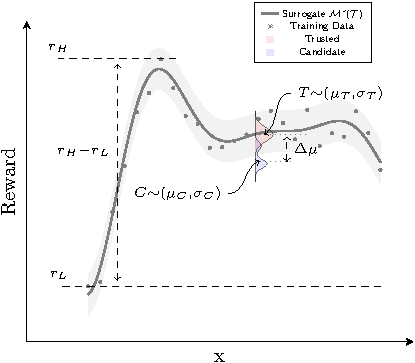
\includegraphics[width=0.8\linewidth]{Figures/sq_v2_fig-crop}
        \caption{Key values involved in calculating \xQ, where $x$ represents a `parameter of interest' for task \task. \nisar{couldn't x also be a solver parameter?}}
        \label{fig:sq_v2}
    \end{figure}